\documentclass[a4paper,twoside,11pt]{book}
\usepackage[amsbb,subscriptcorrection,zswash,mtpcal,mtphrb]{mtpro2}
\usepackage[no-math,cm-default]{fontspec}
\usepackage{xunicode}
\usepackage{xgreek}
\defaultfontfeatures{Mapping=tex-text,Scale=MatchLowercase}
\setmainfont[Mapping=tex-text,Numbers=Lining,Scale=1.0,BoldFont={Tinos Bold}]{Tinos}
\defaultfontfeatures{Ligatures=TeX}
\font\kefalaio="Noto Serif Bold" at 36pt
\font\ArKef="Noto Serif Bold Italic" at 72pt
\font\OnKef="Noto Serif" at 40pt
\font\OnPar="Noto Serif Bold" at 18pt
\font\onoma="URWGothic-Demi" at 11pt
\font\Askhseis="URWGothic-Demi" at 16pt
\newfontfamily\scfont{Nimbus Roman}
\usepackage{fontawesome5}
%\newfontfamily{\FA}{fontawesome.otf}
\usepackage[inner=2.00cm, top=3.00cm, bottom=2.00cm]{geometry}
\geometry{textwidth=12cm,marginparsep=5mm,marginparwidth=5cm}
\usepackage{sidenotes}
\usepackage{amsmath}
\usepackage[amsbb,subscriptcorrection,zswash,mtpcal,mtphrb]{mtpro2}
\usepackage{makeidx}
\usepackage{longtable,varwidth}
\usepackage[usenames,dvipsnames,cmyk,table,x11names]{xcolor}
\definecolor{kefalaio}{cmyk}{0.74,0,0.1,0.47}
\definecolor{portokali}{cmyk}{0,0.54,1,0.08}
\usepackage{float}
\usepackage{subfig}
\def\xrwma{cyan!70!black}
\def\xrwmath{cyan}
\usepackage{etoolbox}
\makeatletter
\newif\ifLT@nocaption
\preto\longtable{\LT@nocaptiontrue}
\appto\endlongtable{%
\ifLT@nocaption
\addtocounter{table}{\m@ne}%
\fi}
\preto\LT@caption{%
\noalign{\global\LT@nocaptionfalse}}
\makeatother
\makeindex
\usepackage{tikz,pgfplots}
\usepackage{tkz-euclide}
\usetikzlibrary{fadings}
\usepackage{wrap-rl}
%\usetkzobj{all}
\usepackage{calc}
\usepackage[colorlinks=false, pdfborder={0 0 0}]{hyperref}
\usepackage{cleveref}
\usepackage[framemethod=tikz]{mdframed}
\definecolor{steelblue}{cmyk}{.7,.278,0,.294}
\definecolor{doc}{cmyk}{1,0.455,0,0.569}
\definecolor{olivedrab}{cmyk}{0.25,0,0.75,0.44}
\usepackage{capt-of}
\usepackage{titletoc}
\usepackage[explicit]{titlesec}
\usepackage{graphicx}
\usepackage{multicol,adjmulticol}
\usepackage{multirow}
\usepackage{enumitem}
\usepackage{tabularx,longtable}
\usepackage[decimalsymbol=comma]{siunitx}
\tikzset{>=latex}
\makeatletter
\pretocmd{\@part}{\gdef\parttitle{#1}}{}{}
\pretocmd{\@spart}{\gdef\parttitle{#1}}{}{}
\makeatother
\usepackage[titletoc]{appendix}
\usepackage{ifthen}
\usepackage{fancyhdr}
\pagestyle{fancy}
\renewcommand{\chaptermark}[1]{\markboth{#1}{}}
\renewcommand{\sectionmark}[1]{\markright{\it\thesection\ #1}}
\makeatletter% so we can use macros with @ in their names
\fancyheadoffset{0cm}
% Set the header/footer width to be the body text block plus the margin
% note area.
\newlength{\overhanglength}
\AtBeginDocument{%
% Calculate the amount to extend the running heads
\setlength{\overhanglength}{\marginparwidth}
\addtolength{\overhanglength}{\marginparsep}

% Set the running head offsets to the overhang length calculated above
\ifthenelse{\NOT\boolean{@mparswitch}\AND\boolean{@twoside}}
{\fancyhfoffset[RE,RO]{\overhanglength}}% asymmetric
{\fancyhfoffset[LE,RO]{\overhanglength}}% symmetric
}
% The running heads/feet don't have rules
\renewcommand{\headrulewidth}{\iftopfloat{0pt}{.5pt}}
\renewcommand{\footrulewidth}{0pt}
\fancyhf{} % clear any existing header and footer fields
% adjust the formatting code to suit your tastes here
\ifthenelse{\boolean{@twoside}}{%
\fancyhead[LE]{\thepage\ $ \cdot $\ \leftmark}%
\fancyhead[RO]{\rightmark\ $ \cdot $\ \thepage}%
}{%
\fancyhead[LE,RO]{\rightmark\quad\thepage}%
}
\makeatother

\usepackage[most]{tcolorbox}
\newcounter{orismos}[chapter]
\renewcommand{\theorismos}{\thechapter.\arabic{orismos}}   
\newcommand{\Orismos}{\refstepcounter{orismos}{\textbf{\textbf{\textcolor{\xrwma}{{\large \onoma{Ορισμός}\hspace{2mm}\theorismos}}}}}\hspace{1mm}}{}
%----------- ΟΡΙΣΜΟΣ------------------
\newenvironment{orismos}[1]
{\begin{tcolorbox}[title=\Orismos:\ \  {\textcolor{black}{\MakeUppercase{\onoma#1}}},breakable,
enhanced standard,titlerule=-.2pt,toprule=0pt, rightrule=0pt, bottomrule=0pt,
colback=white,opacityfill=0,left=2mm,top=1mm,bottom=0mm,
boxrule=0pt,
colframe=white,borderline west={1.5mm}{0pt}{\xrwma},leftrule=2mm,sharp corners,coltitle=\xrwma]}
{\end{tcolorbox}}
%-----------------------------------------

\newcounter{thewrhma}[chapter]
\renewcommand{\thethewrhma}{\thechapter.\arabic{thewrhma}} 
\newcommand{\Thewrhma}{\refstepcounter{thewrhma}{\textbf{\textcolor{LimeGreen!70!black}{{\large \onoma{Θεώρη}μα\hspace{2mm}\thethewrhma}}\hspace{1mm}}}}{}

%----------- ΘΕΩΡΗΜΑ------------------
\newenvironment{thewrhma}[1]
{\begin{tcolorbox}[title=\Thewrhma\ \ :\ \  {\textcolor{black}{\MakeUppercase{\onoma#1}}},breakable,
enhanced standard,titlerule=-.2pt,toprule=0pt, rightrule=0pt, bottomrule=0pt,
colback=white,left=2mm,top=1mm,bottom=0mm,
boxrule=0pt,
colframe=white,borderline west={1.5mm}{0pt}{LimeGreen!70!black},leftrule=2mm,sharp corners,coltitle=LimeGreen!70!black]}
{\end{tcolorbox}}
%-----------------------------------------

%-------- ΠΑΡΑΤΗΡΗΣΕΙΣ -----------------
\newcounter{parathrhsh}[section]
\renewcommand{\theparathrhsh}{\arabic{parathrhsh}}  
\newcommand{\Parathrhsh}[1]{\refstepcounter{parathrhsh}{\textbf{\faExclamationTriangle\ \ -\ \ Παρατήρηση\hspace{2mm}\theparathrhsh}}}{}

%----------- ΠΑΡΑΤΗΡΗΣΗ------------------
\newenvironment{parat}[1]
{\begin{tcolorbox}[title=\Parathrhsh,
breakable,
enhanced standard,lifted shadow={1mm}{-2mm}{3mm}{0.3mm}%
{black!50!white},
colback=red!5!white,
boxrule=0.1pt,
colframe=red!80!black,
fonttitle=\bfseries,width=#1]}
{\end{tcolorbox}}
%-----------------------------------------

\newcounter{porisma}[chapter]
\renewcommand{\theporisma}{\thechapter.\arabic{porisma}}\newcommand{\Porisma}[1]{\refstepcounter{porisma}\textcolor{black}{\textbf{ΠΟΡΙΣΜΑ\hspace{2mm}\theporisma\hspace{1mm} \MakeUppercase{#1}}}\\}{}

\newcounter{protasi}[chapter]
\renewcommand{\theprotasi}{\thechapter.\arabic{protasi}}\newcommand{\Protasi}[1]{\refstepcounter{protasi}\textcolor{black}{\textbf{ΠΡΟΤΑΣΗ\hspace{2mm}\theprotasi\hspace{1mm} \MakeUppercase{#1}}}\\}{}

\usepackage{venndiagram,mathimatika,eurosym}
%-------- ΣΤΥΛ ΚΕΦΑΛΑΙΟΥ ---------
\newcommand*\chapterlabel{}
\newcommand{\fancychapter}{%
\titleformat{\chapter}
{
\normalfont\Huge}
{\gdef\chapterlabel{\thechapter\ }}{0pt}
{\begin{tikzpicture}[remember picture,overlay]
\node[yshift=-9cm] at (current page.north west)
{\begin{tikzpicture}[remember picture, overlay]
%\node[inner sep=0pt] at ($(current page.north) +			(2cm,-0.8in)$) {
\includegraphics[width=21cm]{s}};
\node[anchor=west,xshift=.1\paperwidth,yshift=.14\paperheight,rectangle]
{{\color{white}\fontsize{30}{20}\textbf{\textcolor{black}{\contour{kefalaio}{Κεφάλαιο}}}}};
\node[anchor=west,xshift=.09\paperwidth,yshift=.08\paperheight,rectangle] {\fontsize{44}{20} {\color{black}{{\textcolor{kefalaio}{\contour{white}{\scfont\textsc{##1}}}}}}};
\fill[fill=black] (15.2,2) rectangle (17.8,4.7);
\node[anchor=west,xshift=.74\paperwidth,yshift=.11\paperheight,rectangle]
{{\color{white}\fontsize{80}{20}\textbf{\textit{\textcolor{white}{\contour{black}{\thechapter}}}}}};
\end{tikzpicture}};
\end{tikzpicture}}
\titlespacing*{\chapter}{0pt}{20pt}{100pt}}
%------------------------------------------------
\usepackage[outline]{contour}
\newcommand{\regularchapter}{%
\titleformat{\chapter}[display]
{\normalfont\huge\bfseries}{\chaptertitlename\ \thechapter}{20pt}{\Huge##1}
\titlespacing*{\chapter}
{0pt}{-20pt}{90pt}}
\apptocmd{\mainmatter}{\fancychapter}{}{}
\apptocmd{\backmatter}{\regularchapter}{}{}
\apptocmd{\frontmatter}{\regularchapter}{}{}
\titlespacing*{\section}
{0pt}{30pt}{0pt}
\usepackage{booktabs,colortbl}
\usepackage{hhline}
\DeclareRobustCommand{\perthousand}{%
\ifmmode
\text{\textperthousand}%
\else
\textperthousand
\fi}

\contentsmargin{0cm}
\titlecontents{part}[-1pc]
{\addvspace{10pt}%
\bf\Large ΜΕΡΟΣ\quad }%
{}
{}
{\;\dotfill}%
%------------------------------------------
\titlecontents{chapter}[0pc]
{\addvspace{30pt}%
\begin{tikzpicture}[remember picture, overlay]%
\draw[fill=black,draw=black] (-.3,.5) rectangle (3.7,1.1); %
\pgftext[left,x=0cm,y=0.75cm]{\color{white}\sc\Large\bfseries Κεφάλαιο\ \thecontentslabel};%
\end{tikzpicture}\large\sc}%
{}
{}
{\hspace*{-2.3em}\hfill\normalsize Σελίδα \thecontentspage}%
\titlecontents{section}[2.4pc]
{\addvspace{1pt}}
{\contentslabel[\thecontentslabel]{2pc}}
{}
{\;\dotfill\;\small \thecontentspage}
[]
\titlecontents*{subsection}[4pc]
{\addvspace{-1pt}\small}
{}
{}
{\ --- \small\thecontentspage}
[ \textbullet\ ][]

\makeatletter
\renewcommand{\tableofcontents}{%
\chapter*{%
\vspace*{-20\p@}%
\begin{tikzpicture}[remember picture, overlay]%
\pgftext[right,x=12cm,y=0.2cm]{\Huge\sc\bfseries \contentsname};%
\draw[fill=black,draw=black] (9.5,-.75) rectangle (12.5,1);%
\clip (9.5,-.75) rectangle (15,1);
\pgftext[right,x=12cm,y=0.2cm]{\color{white}\Huge\bfseries \contentsname};%
\end{tikzpicture}}%
\@starttoc{toc}}
\makeatother

\usepackage[contents={},scale=1,opacity=1,color=black,angle=0]{background}

\newcommand\blfootnote[1]{%
\begingroup
\renewcommand\thefootnote{}\footnote{#1}%
\addtocounter{footnote}{-1}%
\endgroup
}
\usepackage{epstopdf}
\epstopdfsetup{update}
\usepackage{textcomp}

\titleformat{\section}
{\normalfont\Large\bf}%
{}{0em}%
{{\color{black}\titlerule[0pt]}\vskip-.2\baselineskip{\parbox[t]{\dimexpr\textwidth-2\fboxsep\relax}{\raggedright\strut\itshape{\LARGE{\fcolorbox{cyan}{cyan}{\textcolor{white}{\thesection}}~\textcolor{cyan}{#1}}}\strut}}}[\vskip 0\baselineskip{\color{cyan}\titlerule[1pt]}]
\titlespacing*{\section}{0pt}{0pt}{30pt}

\titleformat{\subsection}
{\normalfont\large\bf}%
{}{0em}%
{{\color{black}\titlerule[0pt]}\vskip-.2\baselineskip{\parbox[t]{\dimexpr\textwidth-2\fboxsep\relax}{\raggedright\strut\itshape{{\textcolor{magenta!70!black}{\faSquare\ \ \onoma{\MakeUppercase{#1}}}}}\strut}}}[\vskip 0\baselineskip{}]
\titlespacing*{\section}{0pt}{0pt}{30pt}

\newcommand{\methodologia}{\begin{center}
{\large \textbf{ΜΕΘΟΔΟΛΟΓΙΑ}}\\\vspace{-2mm}
\begin{tikzpicture}
\shade[left color=white, right color=black,] (-3cm,0) rectangle (0,.2mm);
\shade[left color=black, right color=white,] (0,0) rectangle (3cm,.2mm);   
\end{tikzpicture}
\end{center}}

\newcommand{\orismoi}{\begin{center}
\vspace{-3mm}{\large \textbf{\textcolor{\xrwma}{ΟΡΙΣΜΟΙ}}}\\\vspace{-2mm}
\begin{tikzpicture}
\shade[left color=white, right color=cyan!80!black,] (-3cm,0) rectangle (0,.2mm);
\shade[left color=cyan!80!black, right color=white,] (0,0) rectangle (3cm,.2mm);   
\end{tikzpicture}
\end{center}}
\newcommand{\thewrhmata}{\begin{center}
{\large \textbf{\textcolor{\xrwmath}{ΘΕΩΡΗΜΑΤΑ - ΠΟΡΙΣΜΑΤΑ - ΠΡΟΤΑΣΕΙΣ\\ΚΡΙΤΗΡΙΑ - ΙΔΙΟΤΗΤΕΣ}}}\\\vspace{-2mm}
\begin{tikzpicture}
\shade[left color=white, right color=\xrwmath,] (-5cm,0) rectangle (0,.2mm);
\shade[left color=\xrwmath, right color=white,] (0,0) rectangle (5cm,.2mm);   
\end{tikzpicture}
\end{center}}
\usepackage[labelfont={footnotesize,it,bf},font={footnotesize},skip=0pt]{caption}

\usepackage{calc,capt-of,hhline,comment}
\makeatletter
\patchcmd{\@caption}{\csname fnum@#1\endcsname:
\ignorespaces#3}{\Centering
\csname fnum@#1\endcsname\ifblank{#3}{}{: \ignorespaces#3}}{}{}
\makeatother 

%----- ΥΠΟΛΟΓΙΣΤΗΣ ----------
%\usepackage{calculator}
%----------------------------

%------ ΜΗΚΟΣ ΓΡΑΜΜΗΣ ΚΛΑΣΜΑΤΟΣ ---------
\DeclareRobustCommand{\frac}[3][0pt]{%
{\begingroup\hspace{#1}#2\hspace{#1}\endgroup\over\hspace{#1}#3\hspace{#1}}}
%----------------------------------------
\usepackage{microtype,changepage}
\usepackage{float}
\usepackage{lipsum}
\tikzstyle{pl}=[line width=0.3mm]
\tikzstyle{plm}=[line width=0.4mm]
%------- ΣΤΥΛ ΠΑΡΑΔΕΙΓΜΑΤΟΣ -------
\newcounter{paradeigma}[chapter]
\renewcommand{\theparadeigma}{\bf\onoma{\thechapter.\arabic{paradeigma}}} 
\newcommand{\Paradeigma}[1]{\refstepcounter{paradeigma}\textcolor{magenta!70!black}{\textbf{{\large \faPlay\ \ \onoma{Παράδειγμα}\hspace{2mm}\theparadeigma\;:\;}\hspace{1mm}}} \MakeUppercase{\onoma{#1}}\\}{}
%-----------------------------------

%------- ΣΤΥΛ ΛΥΣΗΣ ------------------
\newcommand{\lysh}{\textcolor{cyan!80!black}{\onoma{\faCheck\ ΛΥΣΗ}}}
%------------------------------------

%------ ΛΥΜΕΝΑ ΠΑΡΑΔΕΙΓΜΑΤΑ ΤΙΤΛΟΣ ---------
\newcommand{\Lymena}{\begin{center}
\begin{tikzpicture}
\path[left color=cyan!70!black,right color=cyan!80!black,middle color=cyan!80!white] (-7cm,-.6cm) rectangle (6.5cm,.6cm);
\node at (-.25cm,0) {\Large \textcolor{white}{\textbf{ΛΥΜΕΝΑ ΠΑΡΑΔΕΙΓΜΑΤΑ}}};  
\end{tikzpicture}
\end{center}}
%--------------------------------------

%--------- ΑΛΥΤΕΣ ΑΣΚΗΣΕΙΣ ΤΙΤΛΟΣ ----------
\newcommand{\Alyta}{
\begin{tikzpicture}
\path[left color=cyan!70!black,right color=cyan!80!black,middle color=cyan!70!white] (-.3cm,.7cm) --(-.3cm,-.5cm) -- (7.9cm,-.5cm) -- (8.7cm,.63cm) -- (17.2cm,.63cm) -- (17.2cm,.7cm)-- cycle;
\node at (3.8cm,.1) {\LARGE \textcolor{white}{\textbf{\faPenSquare\ \ \rule{.5mm}{5mm}\ \ {\Askhseis{ΑΣΚΗΣΕΙΣ - ΠΡΟΒΛΗΜΑΤΑ}}}}};
\end{tikzpicture}\mbox{}\\}
%--------------------------------------------

%\newcommand{\newgeometria}{
%\newgeometry{inner=2.00cm, top=3.00cm, bottom=2.00cm,outer=1.50cm,textwidth=17.5cm,
%marginparsep=0mm,
%marginparwidth=0cm}
%\fancyhfoffset[LE,RO]{0cm}}
%
%\newcommand{\restoregeometia}{
%\restoregeometry
%\fancyhfoffset[LE,RO]{\overhanglength}}

\newcommand{\full}[1]{\begin{mdframed}[outermargin=\dimexpr-\marginparwidth-\marginparsep\relax,innerleftmargin=0mm,innerrightmargin=0mm,hidealllines=true]
#1
\end{mdframed}}

%\newcommand{\fulltc}[1]{\begin{tcolorbox}[enhanced,breakable, colback=white, colframe=white, check odd page, toggle left and right, grow to right by=\marginparwidth+\marginparsep, toggle enlargement=evenpage]
%#1
%\end{tcolorbox}}

\newcommand{\fulltwoc}[1]{\begin{adjmulticols}{2}{0cm}{\dimexpr-\marginparwidth-\marginparsep\relax}
#1
\end{adjmulticols}}

\usetikzlibrary{shadows,calc}
\usepackage{tcolorbox}
\tcbuselibrary{skins,theorems,breakable}
%---------- ΜΕΘΟΔΟΣ --------------
\newcounter{Methodos}[chapter]
\renewcommand{\theMethodos}{\thechapter.\arabic{Methodos}}
\newenvironment{Methodos}[2][\linewidth]
{\refstepcounter{Methodos}
\begin{tcolorbox}[breakable,
enhanced standard,
boxrule=0.7pt,titlerule=-.2pt,drop fuzzy shadow southeast=black!50,
width=\linewidth,
title style={color=white},
overlay unbroken and first={
\path[left color=cyan!70!black,right color=cyan,draw=black]
([yshift=-\pgflinewidth]frame.north west) to ([yshift=-5pt]title.south west)[rounded corners=2pt] -- ([xshift=-#2-15pt,yshift=-5pt]title.south east) to[rounded corners=2pt] ([xshift=-#2,yshift=-\pgflinewidth]frame.north east) -- cycle;},fonttitle=\bfseries,
before=\par\medskip\noindent,
after=\par\medskip,
toptitle=3pt,
top=11pt,topsep at break=-5pt,
colback=white,title={\large Μέθοδος \theMethodos} : {\textcolor{black}{\MakeUppercase{#1}}}]}
{\end{tcolorbox}}
%------------------------------------------
%---------- ΛΙΣΤΕΣ ----------------------
\newlist{bhma}{enumerate}{3}
\setlist[bhma]{label=\bf\textit{\arabic*\textsuperscript{o}\;Βήμα :},leftmargin=0cm,itemindent=1.5cm,ref=\bf{\arabic*\textsuperscript{o}\;Βήμα}}
\newlist{rlist}{enumerate}{3}
\setlist[rlist]{itemsep=0mm,label=\roman*.}
\newlist{alist}{enumerate}{3}
\setlist[alist]{itemsep=0mm,label=\alph*.}
\makeatletter
\renewrobustcmd{\anw@true}{\let\ifanw@\iffalse}
\renewrobustcmd{\anw@false}{\let\ifanw@\iffalse}\anw@false
\newrobustcmd{\noanw@true}{\let\ifnoanw@\iffalse}
\newrobustcmd{\noanw@false}{\let\ifnoanw@\iffalse}\noanw@false
\renewrobustcmd{\anw@print}{\ifanw@\ifnoanw@\else\numer@lsign\fi\fi}
\makeatother

%----ΣΤΥΛ ΑΣΚΗΣΗΣ ----------
\newcounter{askhsh}[chapter]
\renewcommand{\theaskhsh}{\bf{\textit{{\Large{\thechapter}}.\arabic{askhsh}}}}   
\newcommand{\Askhsh}{\refstepcounter{askhsh}\textcolor{magenta!70!black}{{\theaskhsh}\hspace{2mm}}}{}
%---------------------------

\newlist{brlist}{enumerate}{3}
\setlist[brlist]{itemsep=0mm,label=\bf\roman*.}
\newlist{tropos}{enumerate}{3}
\setlist[tropos]{label=\bf\textit{\arabic*\textsuperscript{oς}\;Τρόπος :},leftmargin=0cm,itemindent=2.3cm,ref=\bf{\arabic*\textsuperscript{oς}\;Τρόπος}}
% Αν μπει το bhma μεσα σε tropo τότε
%\begin{bhma}[leftmargin=.7cm]
\newcommand{\tss}[1]{\textsuperscript{#1}}
\newcommand{\tssL}[1]{\MakeLowercase{\textsuperscript{#1}}}
%------------------------------------------
\setlength{\parindent}{0pt}
\setlist[itemize]{itemsep=0mm}
\tkzSetUpPoint[size=2.8,fill=white]
\newcommand{\twocolkentro}[1]{
\twocolumn[
\begin{@twocolumnfalse}
#1
\end{@twocolumnfalse}]}
\newcommand{\bcc}[1]{
\begin{center}
{\color{\xrwma}{\rule{1cm}{.4pt}}\raisebox{-2.5mm}{\rule{.4pt}{5mm}}}\hspace{1em}\raisebox{-.65ex}{\begin{varwidth}{\dimexpr0.7\textwidth-2em\relax}\centering{\textbf{\textcolor{\xrwma}{\large\scfont\textsc{#1}}}}\end{varwidth}}\hspace*{1em}{\color{\xrwma}{\raisebox{-2.5mm}{\rule{.4pt}{5mm}}\hrulefill}}
\end{center}}

\DeclareMathSizes{10.95}{10.95}{7}{5}
\DeclareMathSizes{6}{6}{3.8}{2.7}
\DeclareMathSizes{8}{8}{5.1}{3.6}
\DeclareMathSizes{9}{9}{5.8}{4.1}
\DeclareMathSizes{10}{10}{6.4}{4.5}
\DeclareMathSizes{12}{12}{7.7}{5.5}
\DeclareMathSizes{14.4}{14.4}{9.2}{6.5}
\DeclareMathSizes{17.28}{17.28}{11}{7.9}
\DeclareMathSizes{20.74}{20.74}{13.3}{9.4}
\DeclareMathSizes{24.88}{24.88}{16}{11.3}

\makeatletter
\AtBeginDocument{
\check@mathfonts
\fontdimen16\textfont2=2.5pt
\fontdimen17\textfont2=2.5pt
\fontdimen14\textfont2=4.5pt
\fontdimen13\textfont2=4.5pt 
}
\makeatother
\newcommand{\bsc}[1]{\textbf{\scfont\textsc{ #1}}}



\begin{document}
\pagestyle{empty}
\frontmatter
\tableofcontents
\restoregeometry % restores the geometry
\mainmatter
\pagestyle{fancy}
\part{Άλγεβρα}
\chapter{Αριθμοι}
\section{Οι αριθμοί}
Το θεμέλιο των μαθηματικών. Αλφάβητο της γλώσσας των μαθηματικών, είναι θα λέγαμε έμφυτη στον ανθρώπινο νου η έννοια των αριθμών, ως εργαλείο μέτρησης.
\begin{marginfigure}[-1cm]
\centering
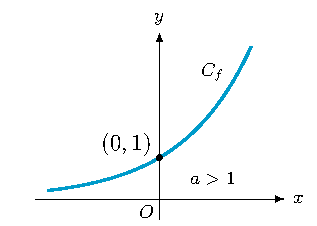
\includegraphics{1}
\caption{Helix}
\end{marginfigure}
\begin{orismos}{Φυσικοί αριθμοί}
Οι φυσικοί αριθμοί είναι $ 0,1,2,3,\ldots $
\end{orismos} 
\begin{thewrhma}{Σύγκριση αριθμών}
Ένας αριθμός $ a $ λέγεται μεγαλύτερος από έναν αριθμό $ \beta $ όταν η διαφορά $ a-\beta $ είναι θετικός αριθμός.
\end{thewrhma}
\begin{marginfigure}[1cm]
\begin{parat}{5cm}
Εκτελούμε όλες τις δυνατές πράξεις ώστε να πούμε αν ο αριθμός είναι ρητός ή όχι. Δηλαδή $ \sqrt{4}=2 $ άρα ρητός.
\end{parat}
\end{marginfigure}
Ο συνδυασμός των περιπτώσεων $ a>\beta $ και $ a=\beta $ συμβολίζεται $ a\geq\beta $ και διαβάζεται $ a $ μεγαλύτερος ίσος του $ \beta $.\\\\
\Paradeigma{Ρητοί αριθμοί}
\bmath{Να βρείτε ποιοί από τους παρακάτω αριθμούς είναι ρητοί.
\[ 2\ \ ,\ \ -3\ \ ,\ \ 9{.}7\ \ ,\ \ \frac{\sqrt{2}}{3}\ \ ,\ \ 2.\bar{3}\ \ ,\ \ -\sqrt{5}\ \ ,\ \ \sqrt{4}\ \ ,\ \ \pi \]}
\lysh\\
\lipsum[1]\mbox{}\\
\Paradeigma{Άρρητοι αριθμοί}
\bmath{Να βρείτε ποιοί από τους παρακάτω αριθμούς είναι άρρητοι.
\[ 2\ \ ,\ \ -3\ \ ,\ \ 9{.}7\ \ ,\ \ \frac{\sqrt{2}}{3}\ \ ,\ \ 2.\bar{3}\ \ ,\ \ -\sqrt{5}\ \ ,\ \ \sqrt{4}\ \ ,\ \ \pi \]}
\lysh\\
\lipsum[1-2]
\subsection{Η ευθεία των αριθμών}
\begin{center}
\begin{tikzpicture}
\draw[-latex] (-5,0)--(5,0)node[xshift=2mm]{\footnotesize$x$};
\foreach \n in {-4.5,-4,...,4.5}{
\draw (\n,-.07)--(\n,.07);
}
\foreach \n in {-4,-3,...,4}{
\draw (\n,-.12)--(\n,.12);
\node at (\n,-.3){\footnotesize$\n$};
}
\foreach \n/\s/\d in {-3.75/{-\frac{15}{4}}/1.4,-1.2/{-1{,}2}/1,0.5/{0{,}5}/1.4,1.4142/\sqrt{2}/1,-2.333/{-2{,}\bar{3}}/1.4,3.14/{\pi}/1.4}{
\draw[-latex,red!70!black] (1.1*\n,.5*\d)node[black,rectangle, fill=red!40,rounded corners=2pt,anchor=south]{\footnotesize$\s$}--(\n,.045);
\fill[red!70!black] (\n,0) circle (1.5pt);}

\foreach \n/\s/\d in {-4/-4/1.4,-0.4/{-0{,}4}/1.4,4/{3{,}\bar{9}}/1.4,2/2/1,0.866/{\frac{\sqrt{3}}{3}}/1,-1.732/{-\sqrt{3}}/1}{
\draw[-latex,red!70!black] (1.1*\n,-.5*\d)node[black,rectangle, fill=red!30,rounded corners=2pt,anchor=north]{\footnotesize$\s$}--(\n,-.045);
\fill[red!70!black] (\n,0) circle (1.5pt);}
\end{tikzpicture}\captionof{figure}{Η ευθεία των πραγματικών αριθμών}
\end{center}
\section{Πράξεις και ιδιότητες}
\full{
\begin{center}
\setlength\arrayrulewidth{1.5pt}\arrayrulecolor{white}
\rowcolors{2}{cyan!70!gray!30}{cyan!10!gray!20}
\begin{tabular}{c|c|c|c}
\hline \rowcolor{cyan!50!gray}\rule[-2ex]{0pt}{5.5ex} \color{white}{\onoma{ΠΡΑΞΗ}} &\color{white} \bsc{Όροι} &\color{white} \bsc{Αποτελεσμα} &\color{white} \bsc{Συμβολισμος} \\ 
\hline \rule[-2ex]{0pt}{5.5ex} \textbf{Πρόσθεση} & Προσθετέοι & Άθροισμα & $ a+\beta $ \\ 
\hline\rule[-2ex]{0pt}{5.5ex} \textbf{Αφαίρεση} & Μειωτέος - Αφαιρετέος & Διαφορά & $ a-\beta $ \\ 
\hline\rule[-2ex]{0pt}{5.5ex} \textbf{Πολλαπλασιασμός} & Παράγοντες & Γινόμενο & $ a\cdot\beta $ \\ 
\hline\rule[-2ex]{0pt}{5.5ex} \textbf{Διαίρεση} & Διαιρετέος - Διαιρέτης & Πηλίκο & $ a:\beta $ \\ 
\hline\hline\end{tabular}\captionof{table}{Βασικές πράξεις}
\end{center}}
\subsection{Δυνάμεις}
\begin{orismos}{Δύναμη πραγματικού αριθμού}
Δύναμη ενός πραγματικού αριθμού $ a $ ονομάζεται το γινόμενο $ \nu $ ίσων παραγόντων του αριθμού αυτού. Συμβολίζεται με $ a^\nu $ όπου $ \nu\in\mathbb{N} $ είναι το πλήθος των ίσων παραγόντων. 
\[ \undercbrace{a\cdot a\cdot\ldots a}_{\nu\textrm{ παράγοντες }}=a^\nu \]
\end{orismos}
Ο αριθμός $ a $ ονομάζεται \textbf{βάση} και ο αριθμός $ \nu $ \textbf{εκθέτης} της δύναμης. Η δύναμη είναι όπως βλέπουμε ένας σύντομος τρόπος να γραφτεί ένας πολλαπλασιασμός όταν οι παράγοντες της είναι ίδιοι. Για παράδειγμα το γινόμενο $ 2\cdot 2\cdot2\cdot2 $ μπορεί να γραφτεί σύντομα ως δύναμη $ 2^4 $. \[ 2\cdot2\cdot2\cdot3\cdot3\cdot3\cdot3=2^3\cdot3^4 \]
\section{Κλάσματα}
\section{Δεκαδικοί αριθμοί}
\section{Απόλυτες τιμές}
\begin{orismos}{Απόλυτη τιμή πραγματικού αριθμού}
Απόλυτη τιμή ενός πραγματικού αριθμού $ a $ ονομάζεται η απόσταση του σημείου $ A(a) $ του αριθμού από την αρχή $ O(0) $ της ευθείας των πραγματικών αριθμών.
\end{orismos}
\begin{center}
\begin{tabular}{c >{\centering\arraybackslash}m{6cm}}
$ |a|=\begin{cases}
\begin{aligned}
a & \;,\;a\geq0\\
-a & \;,\;a<0
\end{aligned}
\end{cases} $  & \begin{tikzpicture}
\draw[-latex] (-1,0) -- coordinate (x axis mid) (4.4,0) node[right,fill=white] {{\footnotesize $ x $}};
\draw (0,.5mm) -- (0,-.5mm) node[anchor=north,fill=white] {{\scriptsize $ 0 $}};
\draw (3,.5mm) -- (3,-.5mm) node[anchor=north,fill=white] {{\scriptsize $ a $}};
\draw[line width=.7mm] (0,0) -- (3,0);
\tkzText(1.5,.34){$ \overcbrace{\rule{28mm}{0mm}}^{{\scriptsize |a|}} $}
\tkzDefPoint(3,0){A}
\tkzDrawPoint(A)
\tkzLabelPoint[above right](A){{\scriptsize $A(a)$}}
\tkzDrawPoint(0,0)
\tkzLabelPoint[above left](0,0){{\scriptsize $O(0)$}}
\end{tikzpicture}
\end{tabular} 
\end{center}
Σύμφωνα με τον ορισμό που δώσαμε, η απόλυτη τιμή ενός θετικού αριθμού $ a $ είναι ίση με τον ίδιο τον αριθμό ενώ ενός αρνητικού αριθμού $ a $ ισούται με τον αντίθετο του δηλαδή $ -a $.
\section{Ρίζες}
\begin{orismos}{Τετραγωνική Ρίζα}
Τετραγωνική ρίζα ενός μη αρνητικού πραγματικού αριθμού $ x $ ονομάζεται ο \textbf{μη αρνητικός} αριθμός $ a $ ο οποίος αν υψωθεί στο τετράγωνο δίνει τον αριθμό $ x $. Συμβολίζεται με $ \sqrt{x} $.
\[ \sqrt{x}=a\;\;,\;\;\textrm{ όπου }x\geq0\textrm{ και }a\geq0 \]
\end{orismos}
Συγκεκριμένα, η ποσότητα που βρίσκεται κάτω από τη ρίζα ονομάζεται \textbf{υπόριζο}, ενώ σύμφωνα με τον ορισμό της ρίζας δεν ορίζεται, στο σύνολο $ \mathbb{R} $ των πραγματικών αριθμών, η τετραγωνική ρίζα ενός αρνητικού αριθμού.\\\\
\Paradeigma{Υπολογισμός τετραγωνικής ρίζας}
\bmath{Να υπολογίσετε τις ακόλουθες τετραγωνικές ρίζες.
\begin{multicols}{3}
\begin{rlist}
\item $ \sqrt{25} $
\item $ \sqrt{144} $
\item $ \sqrt{0{,}16} $
\end{rlist}
\end{multicols}}
\lysh
\begin{rlist}
\item $ \sqrt{25}=5 $ διότι $ 5^2=25 $.
\item $ \sqrt{144}=12 $ γιατί $ 12^2=144 $.
\item $ \sqrt{0{,}16}=0{,}4 $ διότι $ 0{,}4^2=0{,}16 $.
\end{rlist}
\begin{orismos}{ριζα \MakeLowercase{ν}-ταξης πραγματικού αριθμού}
Ρίζα $ \nu $-οστής \textbf{τάξης} ενός μη αρνητικού αριθμού $ x $ ονομάζεται ο \textbf{μη αρνητικός} αριθμός $ a $ που αν υψωθεί στη δύναμη $ \nu $ δίνει αποτέλεσμα $ x $ (υπόριζο). Συμβολίζεται με $ \sqrt[\nu]{x} $.
\[ \sqrt[\nu]{x}=a\;\;,\;\;\textrm{ όπου }x\geq0\textrm{ και }a\geq0 \]
\end{orismos}
\Paradeigma{Υπολογισμός \MakeLowercase{ν}-οστής ρίζας}
\bmath{Να υπολογίσετε τις ακόλουθες τετραγωνικές ρίζες.
\begin{multicols}{3}
\begin{rlist}
\item $ \sqrt[3]{27} $
\item $ \sqrt[4]{256} $
\item $ \sqrt[7]{128} $
\end{rlist}
\end{multicols}}
\lysh
\begin{rlist}
\item $ \sqrt[3]{27}=3 $ διότι $ 3^3=27 $
\item $ \sqrt[4]{625}=5 $ διότι $ 5^4=625 $
\item $ \sqrt[7]{128}=2 $ διότι $ 2^7=128 $
\end{rlist}
\begin{thewrhma}{Ιδιότητες τετραγωνικής ρίζας}
\begin{alist}
\item $ \left(\sqrt{x}\right)^2=x $ για κάθε $ x\geq0 $.
\item $ \sqrt{x^2}=|x| $ για κάθε $ x\in\mathbb{R} $.
\end{alist}
\end{thewrhma}
Οι ιδιότητες των ριζών φαίνονται στον παρακάτω πίνακα...
\textbf{Ιδιότητες Ριζών}\\
Για κάθε $ x,y\in\mathbb{R} $ πραγματικούς αριθμούς και $ \nu,\mu,\rho\in\mathbb{N} $ φυσικούς αριθμούς ισχύουν οι παρακάτω ιδιότητες για την τετραγωνική και ν-οστή ρίζα τους.
\vspace{-5mm}
\begin{center}
\setlength\arrayrulewidth{1.5pt}\arrayrulecolor{white}
\rowcolors{2}{cyan!70!gray!30}{cyan!10!gray!20}
\begin{longtable}{c|c}
\hline \rowcolor{cyan!50!gray}\rule[-2ex]{0pt}{5.5ex} \textbf{Ιδιότητα} & \textbf{Συνθήκη} \\
\hhline{--}\rule[-2ex]{0pt}{5.5ex}  Τετράγωνο ρίζας & $ \left(\sqrt{x}\;\right)^2=x\;\;,\;\; x\geq0  $ \\
\hline\rule[-2ex]{0pt}{5.5ex}  Ν-οστή δύναμη ν-οστής ρίζας & $ \left(\sqrt[\nu]{x}\;\right)^\nu=x\;\;,\;\; x\geq0  $ \\
\hline\rule[-2ex]{0pt}{5.5ex} Ρίζα τετραγώνου & $ \sqrt{x^2}=|x|\;\;,\;\; x\in\mathbb{R} $\\
\hline\rule[-2ex]{0pt}{7ex}  Ν-οστή ρίζα ν-οστής δύναμης & \begin{minipage}{5.7cm}
$ \sqrt[\nu]{x^\nu}=\ccases{\hiderowcolors
|x|&  x\in\mathbb{R}\textrm{ αν }\nu\textrm{ άρτιος}\\x&  x\geq0\textrm{ και } \nu\in\mathbb{N}} $
\end{minipage}\\
\hhline{~-} \rowcolor{cyan!70!gray!30}  & $ \sqrt{x\cdot y}=\sqrt{x}\cdot\sqrt{y}\;\;,\;\; x,y\geq0 $ \rule[-2ex]{0pt}{5.5ex}\\
\rule[-2ex]{0pt}{5.5ex}\multirow{-3}{*}{Ρίζα γινομένου} & $ \sqrt[\nu]{x\cdot y}=\sqrt[\nu]{x}\cdot\sqrt[\nu]{y}\;\;,\;\; x,y\geq0 $ \\
\hhline{~-} \rowcolor{cyan!10!gray!20} & $ \sqrt{\dfrac{x}{y}}=\dfrac{\sqrt{x}}{\sqrt{y}}\;\;,\;\; x\geq0\textrm{ και }y>0 $ \rule[-2ex]{0pt}{6.5ex}\\
\rule[-2ex]{0pt}{7.5ex}\multirow{-4}{*}{Ρίζα πηλίκου} & $ \sqrt[\nu]{\dfrac{x}{y}}=\dfrac{\sqrt[\nu]{x}}{\sqrt[\nu]{y}}\;\;,\;\; x\geq0\textrm{ και }y>0 $ \\
\hhline{~-}\rowcolor{cyan!70!gray!30}\rule[-2ex]{0pt}{5.5ex} Μ-οστή ρίζα ν-οστής ρίζας  & $ \sqrt[\mu]{\sqrt[\nu]{x}}=\sqrt[\nu\cdot\mu]{x}\;\;,\;\; x\geq0 $ \\
\hline\rowcolor{cyan!10!gray!20}\rule[-2ex]{0pt}{5.5ex} Απλοποίηση ρίζας & $ \sqrt[\nu]{x^\nu\cdot y}=x\sqrt[\nu]{y}\;\;,\;\; x,y\geq0  $ \\
\hline\rowcolor{cyan!70!gray!30}\rule[-2ex]{0pt}{5.5ex} Απλοποίηση τάξης και δύναμης & $ \sqrt[\mu\cdot\rho]{x^{\nu\cdot\rho}}=\sqrt[\mu]{x^{\nu}}\;\;,\;\; x\geq0 $ \\
\hline
\end{longtable}\captionof{table}{Ιδιότητες ριζών}
\end{center}
\begin{orismos}{Δύναμη με ρητό έκθετη}
Δύναμη ενός \textbf{θετικού} αριθμού $ a $ με εκθέτη ένα ρητό αριθμό $ \frac{\mu}{\nu} $, με $ \mu\in\mathbb{Z} $ και $ \nu\in\mathbb{N}^* $, είναι η ρίζα $ \nu $-τάξης του αριθμού $ a $ υψωμένο στον εκθέτη $ \mu $.
\[ a^{\frac{\mu}{\nu}}=\sqrt[\nu]{a^\mu}\ ,\ \textrm{ όπου } a>0 \]
\end{orismos}
\Paradeigma{Δυνάμεις με ρητό εκθέτη}
\bmath{Να γραφτούν οι ακόλουθες δυνάμεις με μορφή ρίζας.
\begin{multicols}{2}
\begin{rlist}
\item $ 3^{\frac{1}{2}} $
\item $ 8^{\frac{2}{3}} $
\end{rlist}
\end{multicols}}
\lysh
\begin{rlist}
\item Στο κλάσμα $ \frac{1}{2} $ στον εκθέτη της δύναμης, το $ 1 $ αντιστοιχεί στον εκθέτη της βάσης $ 3 $ και ο αριθμός $ 2 $ παριστάνει την τάξη της ρίζας, άρα πρόκειται για τετραγωνική. Συμβολικά θα είναι
\[ 3^{\frac{1}{2}}=\sqrt[2]{3^1}=\sqrt{3} \]
\item Ομοίως με το προηγούμενο παράδειγμα, αριθμητής και παρονομαστής του $ \frac{2}{3} $ αντιστοιχούν σε εκθέτη και τάξης ρίζας και θα έχουμε
\[ 8^{\frac{2}{3}}=\sqrt[3]{8^2}=\sqrt[3]{64}=4 \]
\end{rlist}
\section{Συστήματα αρίθμησης}
\lipsum\noindent
\full{\Alyta}\vspace{-14mm}
\fulltwoc{\Askhsh Να επιλύσετε με τη μέθοδο της αντικατάστασης το παρακάτω γραμμικό σύστημα $ 3\times 3 $.
\[ \csysteme{2x-y=3,x+3y=5,3x-4y+z=9} \]
\Askhsh να εξετάσετε ποιοι από τους παρακάτω αριθμούς είναι ρητοί και ποιοι άρρητοι
\[ \sqrt{2}, \frac{1}{\sqrt{4}},\ln{e},\pi \]
\Askhsh \[ \sqrt{3},\ln{2e},\frac{\sqrt{9}}{2},\pi^2 \]
\Askhsh Να λυθεί η παρακάτω εξίσωση με τη βοήθεια του σχήματος Horner. \[ x^3-2x^2-4x+8=0 \]
\Askhsh Να υπολογιστεί το ολοκλήρωμα \[ \int_{0}^{1}{x\ln{x}dx} \]
\lipsum[1-20]}
\chapter{Λογική - Προτασιακός Λογισμός}
\chapter{Αλγεβρικές παραστάσεις}
\section{Γενικά}
\section{Πολυώνυμα}
\[ P(x)=x^2-3x+4 \]
\section{Ρητές}
\section{Άρρητες}
\lipsum[1-20]
\chapter{Σύνολα}
\section{Η έννοια του συνόλου}
\begin{orismos}{Σύνολο} 
Σύνολο ονομάζεται μια συλλογή όμοιων αντικειμένων, τα οποία είναι καλά ορισμένα και διακριτά μεταξύ τους.
\end{orismos}
\begin{itemize}[itemsep=0mm]
\item Τα αντικείμενα ενός συνόλου ονομάζονται \textbf{στοιχεία}.
\item Τα σύνολα τα συμβολίζουμε με ένα κεφαλαίο γράμμα.
\item Για να δηλώσουμε ότι ένα στοιχείο $ x $ \textbf{ανήκει} σε ένα σύνολο $ A $ γράφουμε $ x\in A $. Ενώ αν το $ x $ \textbf{δεν ανήκει} στο σύνολο $ A $ γράφουμε $ x\notin A $.
\item \textbf{Κενό} ονομάζεται το σύνολο που δεν έχει κανένα στοιχείο. Συμβολίζεται με $ \varnothing $ ή $ \left\lbrace \right\rbrace  $.
\item \textbf{Βασικό} ονομάζεται το σύνολο ......(να μπει αλλού)
\end{itemize}
\subsection{ΒΑΣΙΚΑ ΣΥΝΟΛΑ ΑΡΙΘΜΩΝ}
\begin{enumerate}[itemsep=0mm,label=\bf\arabic*.]
\item \textbf{Φυσικοί Αριθμοί} : Οι αριθμοί $ 0,1,2,\ldots $. Το σύνολο των φυσικών συμβολίζεται με $ \mathbb{N} $ και είναι : $ \mathbb{N}=\{0,1,2,\ldots\} $.
\item \textbf{Ακέραιοι Αριθμοί} : Το σύνολο των φυσικών αριθμών μαζί με τους αντίθετους τους. Συμβολίζεται με $ \mathbb{Z} $ και είναι : $ \mathbb{Z}=\{\ldots,-2,-1,0,1,2,\ldots\} $.
\item \textbf{Ρητοί Αριθμοί} : Οι αριθμοί που μπορούν να γραφτούν στη μορφή κλάσματος με ακέραιους όρους. Το σύνολο των ρητών συμβολίζεται με $ \mathbb{Q} $ και είναι : \[ \mathbb{Q}=\left\lbrace \left. \frac{a}{\beta}\right|a,\beta\in\mathbb{Z},\beta\neq0\;\right\rbrace. \]
\item \textbf{Άρρητοι Αριθμοί} : Κάθε αριθμός ο οποίος δεν είναι ρητός. Κατά κύριο λόγο, άρρητοι αριθμοί είναι οι ρίζες που δεν έχουν ρητό αποτέλεσμα, ο αριθμός $ \pi $ και άλλοι που θα συναντήσουμε στη συνέχεια.
\item \textbf{Πραγματικοί Αριθμοί} : Οι ρητοί μαζί με τους άρρητους μας δίνουν τους πραγματικούς αριθμούς... Συμβολίζεται με $ \mathbb{R} $ και είναι : $ \mathbb{R}= $ $ \{ $όλοι οι αριθμοί$ \} $.
\end{enumerate}
Τα παραπάνω σύνολα \textbf{χωρίς το μηδέν} συμβολίζονται αντίστοιχα με $ \mathbb{N}^*,\mathbb{Z}^*,\mathbb{Q}^*,\mathbb{R}^*$.\\\\
\Paradeigma{Στοιχείο συνόλου}
\bmath{Να εξετάσετε αν οι παρακάτω προτάσεις είναι σωστές ή λανθασμένες.
\begin{multicols}{4}
\begin{rlist}
\item $ 2\in\mathbb{Z} $
\item $ -3\in\mathbb{N} $
\item $ \dfrac{4}{5}\in\mathbb{R} $
\item $ \sqrt{3}\in\mathbb{Q} $
\item $ 0\in\mathbb{R} $
\item $ 7\in\mathbb{N} $
\item $ 1{,}3\in\mathbb{Q} $
\item $ 0{,}\bar{1}\in\mathbb{Q} $
\item $ \sqrt{9}\in\mathbb{N} $
\item $ (\sqrt{2})^2\notin\mathbb{Z} $
\end{rlist}
\end{multicols}}
\section{Πράξεις μεταξύ συνόλων}
\[ A\cup B=\{x\in\Omega : x\in A\textrm{ ή }x\in B \} \]
\[ A\cap B=\{x\in\Omega : x\in A\textrm{ και } x\in B \} \]
\[ A'=\{x\in \Omega : x\notin A\} \]
\[ A-B=\{x\in\Omega : x\in A\textrm{ και }x\notin B\} \]
\chapter{Τριγωνομετρία}
\section{Η έννοια των τριγωνομετρικών αριθμών}
\begin{orismos}{Ημίτονο}
Ημίτονο μιας οξείας γωνίας ενός ορθογωνίου τριγώνου ονομάζεται ο λόγος της απέναντι κάθετης πλευράς προς την υποτείνουσα.
\[ \textrm{Ημίτονο}=\frac{\textrm{Απέναντι Κάθετη}}{\textrm{Υποτείνουσα}}\;\;,\;\;\hm{\omega}=\frac{A\varGamma}{B\varGamma} \]
\end{orismos}
\begin{marginfigure}[-4cm]
\begin{tikzpicture}[scale=.8]
\tkzDefPoint(0,0){A}
\tkzDefPoint(3,0){B}
\tkzDefPoint(0,4){C}
\tkzMarkAngle[fill=\xrwma!50,size=.5](C,B,A)
\tkzMarkRightAngle[size=.3](B,A,C)
\tkzDrawPolygon[pl](A,B,C)
\tkzText(2.2,.3){$ \omega $}
\tkzLabelPoint[left](A){$ A $}
\tkzLabelPoint[right](B){$ B $}
\tkzLabelPoint[left](C){$ \varGamma $}
\tkzDrawPoints(A,B,C)
\node[rotate=-53.13] at(1.7,2.2){{\footnotesize Υποτείνουσα}};
\node[rotate=90] at(-.3,2){{\footnotesize Απέναντι κάθετη}};
\node at(1.5,-.4){{\footnotesize Προσκείμενη κάθετη}};
\end{tikzpicture}\captionof{figure}{Τριγωνομετρικοί αριθμοί οξείας γωνίας}
\end{marginfigure}
\section{Ο τριγωνομετρικός κύκλος}
\section{Τριγωνομετρικές ταυτότητες}
\[ \hm^2{x}+\syn^2{x}=1 \]
\section{Νόμος ημιτόνων - συνημιτόνων}
\section{Αναγωγή στο 1ο τεταρτημόριο}
\chapter{Εξισώσεις - Ανισώσεις}
\section{Ισότητες}
\section{Διάταξη}
\begin{orismos}{Εξίσωση}
Εξίσωση ονομάζεται κάθε ισότητα η οποία περιέχει μεταβλητές.
\end{orismos}
\section{Πολυωνυμικές 1ου βαθμού}
\subsection{Εξισώσεις}
\[ ax+\beta=0 \]
\Paradeigma{}
\bmath{Να λυθεί η εξίσωση $ 3x-12=0 $}\\
\lysh
\begin{align*}
3x-12&=0\Rightarrow\\
3x&=12\Rightarrow\\
\frac{3x}{3}&=\frac{12}{3}\Rightarrow\\
x&=4
\end{align*}
\[ \frac{x-1}{3}+\frac{2x+3}{4}=1-\frac{5x-8}{12} \]
\lysh
\begin{align*}
\frac{x-1}{3}+\frac{2x+3}{4}&=1-\frac{5x-8}{12}\Rightarrow\\
12\cdot\frac{x-1}{3}+12\cdot\frac{2x+3}{4}&=12\cdot 1-12\cdot\frac{5x-8}{12}\Rightarrow\\
4(x-1)+3(2x+3)&=12-(5x-8)\Rightarrow\\
4x-4+6x+9&=12-5x+8\Rightarrow\\
4x+6x+5x&=12+4-9+8\Rightarrow\\
15x&=15\Rightarrow \frac{15x}{15}=\frac{15}{15}\Rightarrow\\x&=1
\end{align*}
\subsection{Ανισώσεις}
\[ 4x-12<0 \]
\[ \sum_{n=1}^{\infty}{\frac{(-1)^n}{n^2}}=\frac{\pi^2}{12} \]
\[ 2x+8>4x-12 \]
\section{Πολυωνυμικές 2ου βαθμού}
\Paradeigma{Ανίσωση 2\tssL{ου} βαθμού}
\bmath{Να βρεθούν οι λύσεις της παρακάτω ανίσωσης
\[ x^2-4x+3\leq 0 \]}
\lysh
\[ x^2-4x+3\leq 0 \]
\section{Πολυωνυμικές 3ου βαθμού}
\[ ax^3+\beta x^2+\gamma x+\delta=0 \]

\section{Πολυωνυμικές 4ου βαθμού}
\section{Γενικές Πολυωνυμικές}
\section{Κλασματικές}
\section{Άρρητες}
\[ \sqrt{x-1}=3\Rightarrow x-1=9\Rightarrow x=10 \]
\section{Συστήματα εξισώσεων}
\subsection{Γραμμικές εξισώσεις}
\[ ax+\beta y=\gamma \]
\subsection{Συστήματα}
\begin{orismos}{Γραμμικό σύστημα $ \mathbold{2\times2} $}
Γραμμικό σύστημα δύο εξισώσεων με δύο άγνωστους ονομάζεται ο συνδυασμός - σύζευξη δύο γραμμικών εξισώσεων. Είναι της μορφής :
\[ \ccases{ax+\beta y=\gamma\\a'x+\beta'y=\gamma'} \]
\end{orismos}
Οι πραγματικοί αριθμοί $ a,a',\beta,\beta' $ ονομάζονται \textbf{συντελεστές} του συστήματος, ενώ οι $ \gamma, \gamma' $ είναι οι \textbf{σταθεροί όροι} του. Όπως είδαμε και προηγουμένως, η λύση μιας γραμμικής εξίσωσης είναι ένα ζεύγος αριθμών. Κατ' αναλογία λοιπόν με τις εξισώσεις αυτές, οι λύσεις που αναζητούμε για ένα $ 2\times2 $ γραμμικό σύστημα έχουν την ίδια ακριβώς μορφή και δίνονται από τον ακόλουθο ορισμό:
\begin{orismos}{Λύσεις γραμμικού συστήματος $ \mathbold{2\times2} $}
Λύση ενός $ 2\times 2 $ γραμμικού συστήματος ονομάζεται κάθε ζεύγος αριθμών $ (x_0,y_0) $ που επαληθεύει και τις δύο εξισώσεις του.
\end{orismos}
\begin{thewrhma}{Επίλυση συστήματος {$ \mathbold{2\mathbold{\times}2} $} με ορίζουσες}
Έστω το γραμμικό σύστημα 
\[ \ccases{{a}x+{\beta} y={\gamma}\\{a'}x+{\beta'} y={\gamma'} } \]
με πραγματικούς συντελεστές και ορίζουσα συντελεστών $ D $.
\begin{rlist}
\item Αν $ D\neq0 $ τότε το σύστημα έχει μοναδική λύση. Οι τιμές των μεταβλητών δίνονται από τις σχέσεις
\[ x=\frac{D_x}{D}\;\;,\;\;y=\frac{D_y}{D} \]
ενώ η λύση του συστήματος θα είναι $ (x,y)=\left(\frac{D_x}{D},\frac{D_y}{D} \right)  $.
\item Αν $ D=0 $ τότε το σύστημα είναι είτε αόριστο είτε αδύνατο. Συγκεκριμένα:
\begin{alist}
\item αν $ D_x\neq0 $ ή $ D_y\neq0 $ τότε το σύστημα είναι αδύνατο.
\item αν $ D_x=0 $ και $ D_y=0 $ τότε το σύστημα είναι αόριστο.
\end{alist}
\end{rlist}
\end{thewrhma}
\chapter{Ακολουθίες}
\section{Βασικές έννοιες}
\section{Αριθμητική πρόοδος}
\begin{orismos}{Αριθμητική πρόοδος}
Μια ακολουθία $ (a_{\nu}) $ ονομάζεται αριθμητική πρόοδος αν κάθε όρος της προκύπτει από τον προηγούμενο, προσθέτοντας ένα σταθερό αριθμό $ \omega $.
\end{orismos}
\[ a_{\nu+1}=a_{\nu}+\omega\ \ ,\ \ \nu=1,2,\ldots \]
\[ a_{\nu}=a_1+(\nu-1)\omega \]
\[ S_{\nu}=\frac{\nu}{2}\left(a_1+a_{\nu}\right)=\frac{\nu}{2}\left[2a_1+(\nu-1)\omega\right] \]
\section{Γεωμετρική πρόοδος}
\[ a_{\nu}=\lambda\cdot a_{\nu}\ \ ,\ \ \nu=1,2,\ldots \]
\[ a_{\nu}=a_1\lambda^{\nu-1} \]
\[ S_{\nu}=a_1\frac{\lambda^{\nu}-1}{\lambda-1} \]
\section{Αρμονική πρόοδος}
\[ \int_{-1}^{1}{\log{x}\d x} \]
\chapter{Συστήματα εξισώσεων - ανισώσεων}
\section{Γραμμική εξίσωση}
\[ ax+\beta y=\gamma \]
\[ a_1x_1+a_2x_2+\ldots+a_{\nu}x_{\nu}=\beta \]
\section{Γραμμικά συστήματα $ 2\times 2 $}
\[ \systeme[xy]{{a}x+{\beta}y=\gamma, {a}x+{\beta} y=\gamma} \]
\[ x=\frac{D_x}{D}\ \ y=\frac{D_y}{D} \]
\section{Γραμμικά συστήματα $ 3\times 3 $}
\chapter{Εκθετική συνάρτηση - Λογάριθμος}
\[ x=\log_{a}{\theta} \]
\[ \int_{-1}^{1}{f(x)\d x} \]
\chapter{Μιγαδικοί αριθμοί}
\[ i^2=-1 \]
\[ \mathbb{C}=\{z=a+\beta i\ :\ a,\beta\in\mathbb{R}\} \]
\[ \Re{z}=a\ \ ,\ \ \Im{z}=\beta \]
\section{Πράξεις με μιγαδικούς}
\subsection{Πρόσθεση - Αφαίρεση μιγαδικών}
\[ z_1+z_2=\left(a_1+\beta_1 i\right)+\left(a_2+\beta_2 i\right)=a_1+a_2+\left(\beta_1+\beta_2\right)i \]
\chapter{Πίνακες}
\[ A=\begin{pmatrix}
a_{11} & a_{12} & \ldots & a_{1\nu}\\
a_{21} & a_{22} & \ldots & a_{2\nu}\\
\vdots & \vdots & \ddots & \vdots\\
a_{\nu 1} & a_{\nu 2} & \ldots & a_{\nu\nu}
\end{pmatrix} \]
\[ \int_{a}^{\beta}{f(x)\d x} \]
\part{Ανάλυση}
\chapter{Η έννοια της συνάρτησης - Βασικές συναρτήσεις}
\begin{orismos}{Συνάρτηση}
Συνάρτηση από ένα σύνολο $ A $ σε ένα σύνολο $ B $ ονομάζεται μια διαδικασία (αντιστοίχηση) με την οποία κάθε στοιχείο $ x\in A $ αντιστοιχεί σε ένα μόνο στοιχείο $ y\in B $.
\end{orismos}
\[ f:A\to B \]
\[ y=f(x)\ ,\ x\in D_f \]
\[ f(D_f) \]
\chapter{Όρια}
\[ \lim_{x\to x_0}{f(x)}=l \]
\[ \lim_{x\to x_0^-}{f(x)}=l_1 \]
\[ \lim_{x\to x_0^+}{f(x)}=l_2 \]
\chapter{Παράγωγοι}
\[ f'(x_0)=\lim_{x\to x_0}{\frac{f(x)-f(x_0)}{x-x_0}} \]
\[ f'(x_0)=\lim_{h\to 0}\frac{f(x_0+h)-f(x_0)}{h} \]
\chapter{Ολοκληρώματα}
\[ \int_{a}^{\beta}{f(x)\d x}=F(\beta)-F(a) \]
\[ \int_{-\infty}^{\infty}{f(x)\d x}=\lim_{c\to \infty}{\int_{-c}^{c}{f(x)\d x}} \]
\chapter{Διαφορικές Εξισώσεις 1\tss{ης} τάξης}
\chapter{Διαφορικές εξισώσεις 2\tss{ης} τάξης}
\chapter{Ολοκληρωτικές εξισώσεις}
\chapter{Μερικές διαφορικές εξισώσεις 1ης τάξης}
\[ a_1u_x+a_2u_y=\beta_1 \]
\chapter{Μερικές διαφορικές εξισώσεις 2ης τάξης}
\begin{tikzpicture}[remember picture,overlay]
\node[yshift=-13cm] at (current page.north west)
{\begin{tikzpicture}[remember picture, overlay]
\node[inner sep=0pt] at ($(current page.north) +			(2cm,-0.8in)$) {
\includegraphics[width=21cm]{p}};
\end{tikzpicture}};
\end{tikzpicture}
\begin{orismos}{Σειρά Fourier}
Έστω $ f\in E $. Η ακόλουθη σειρά λέγεται σειρά Fourier
της $ f $
\[ f(x)=\frac{a_0}{2}+\sum_{n=1}^{\infty}{(a_n\cos{(nx)}+b_n\sin{(nx)})} \]
όπου $ a_n,b_n $ με $ n=1,2,\ldots $ είναι οι συντελεστές Fourier και ορίζονται ως εξής:
\[ a_n=\frac{1}{\pi}\int_{-\pi}^{\pi}{f(x)\cos{(nx)}}\d x\ \ \textrm{και}\ \ b_n=\frac{1}{\pi}\int_{-\pi}^{\pi}{f(x)\sin{(nx)}}\d x \]
\end{orismos}
\begin{thewrhma}{Κλειστότητα και ισότητα του Parseval}
Ένα άπειρο ορθοκανονικό σύστημα $ \{e_1, e_2,\ldots\}\subset H $ είναι κλειστό στον $ H $, αν και μόνο αν, για κάθε $ x\in H $ ισχύει
\[ \left\| x\right\|^2=\sum_{i=1}^{n}{|(x,e_i)|^2}. \]
Η παραπάνω σχέση λέγεται ισότητα του Parseval.
\end{thewrhma}
\chapter{Μελέτη συνάρτησης}
\section{Μονοτονία - ακρότατα}
\section{Κυρτότητα}
\section{Ασύμπτωτες}
\chapter{Συνέχεια συνάρτησης}
\begin{orismos}{Συνέχεια συνάρτησης σε σημείο}
Μια συνάρτηση $ f $ θα λέγεται συνεχής σε ένα σημείο $ x_0 $ του πεδίου ορισμού της αν το όριο της στο $ x_0 $ ισούται με την τιμή της στο σημείο αυτό.
\[ \lim_{x\to x_0}{f(x)}=f(x_0) \]
\end{orismos}
\begin{orismos}{Συνεχής συνάρτηση}
Μια συνάρτηση $ f $ θα λέγεται συνεχής στο πεδίο ορισμού της ή απλά συνεχής, εάν είναι συνεχής σε κάθε σημείο $ x_0 $ του πεδίου ορισμού της.
\end{orismos}
\chapter{Μιγαδική ανάλυση}
\part{Γεωμετρία}
\chapter{Συστήματα συντεταγμένων}
\begin{tikzpicture}[remember picture,overlay]
\node[yshift=-11cm] at (current page.north west)
{\begin{tikzpicture}[remember picture, overlay]
\node[inner sep=0pt] at ($(current page.north) +			(2cm,-0.8in)$) {
\includegraphics[width=21cm]{s}};
\end{tikzpicture}};
\end{tikzpicture}
\section{Καρτεσιανές 2Δ}
\section{Πολικές}
\[ (x,y)=(\rho\cos{\theta},\rho\sin{\theta}) \]
\begin{center}
\begin{tikzpicture}[scale=0.64]
%Circles 
\foreach \r in {1, 2,...,7}
\draw[SteelBlue3, thick] (0,0) circle (\r);    
\foreach \r in {0.5, 1.5,...,7}
\draw[Azure4, thin] (0,0) circle (\r);
%1° Rays
\foreach \a in {0, 1,...,359}
\draw[Azure4] (\a:7.7) -- (\a:8);
%5° Rays
\foreach \a in {0, 5,...,359}
\draw[Azure4] (\a:7.5) -- (\a:8);      
%15° Rays
\foreach \a in {0, 15,...,359}
\draw[thick,Azure4] (\a:1) -- (\a:8); 
%30° Rays
\foreach \a in {0, 30,...,359}
\draw[thick,Azure4] (0, 0) -- (\a:8);
%Main rays
\draw (-8,0) -- (8,0);
\draw (0,-8) -- (0,8);
%Angle labels  
\foreach \a in {0, 15,...,359}
\draw (\a: 8.5) node[fill=white,inner sep=.2mm] {$\a^\circ$};
%Central point
\draw[fill=black] (0,0) circle(0.7mm);
%Radius labels (background filled white)
\foreach \r in {0,1,...,7}
\draw (\r,0) node[inner sep=1pt,below=3pt,rectangle,fill=white] {$\r$};
\end{tikzpicture}
\end{center}
\section{Καρτεσιανές 3Δ}
\section{Κυλινδρικές}
\section{Σφαιρικές}
\section{Καρτεσιανές}
\chapter{Διανύσματα}
\chapter{Ευθεία - Γωνίες}
\chapter{Κύκλος}
\chapter{Πολύγωνα - Κανονικά πολύγωνα}
\chapter{Αναλογίες - Ομοιότητα}
\chapter{Στερεομετρία}
\chapter{Βασικά θεωρήματα στα τρίγωνα}
\section{Πυθαγόρειο θεώρημα}
\section{Θεώρημα Θαλή}
\section{Θεώρημα διχοτόμων}
\section{Θεώρημα διαμέσων}
\chapter{Παραλληλόγραμμα}
\chapter{Τρίγωνα}
\chapter{Κωνικές τομές}

\part{Πιθανότητες - Στατιστική}
\chapter{Βασικές έννοιες της στατιστικής}
\chapter{Η έννοια της πιθανότητας}
\end{document}
